\lipsum[2]
 

% image4
% Figure X. Distribution of the protocol\_type feature in the training set (top 3 categories). TCP dominates the dataset, while UDP and ICMP occur far less frequently, illustrating the categorical imbalance present in NSL-KDD.
\begin{figure}[H]
\centering
  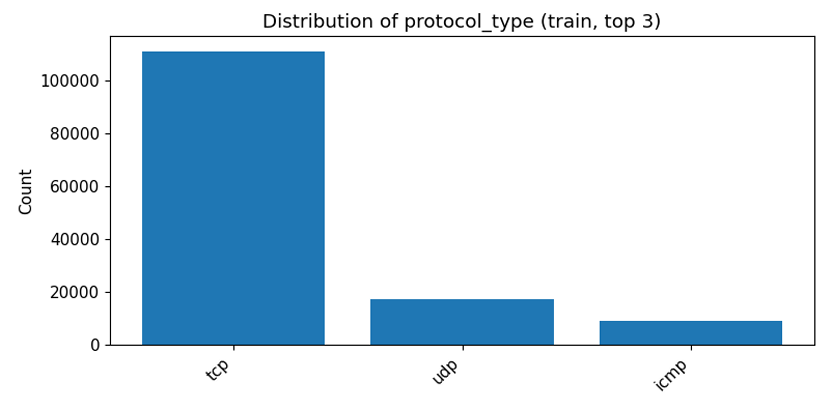
\includegraphics[width=\linewidth]{Figures/methodologyfigures/image4.png}
  \caption{Distribution of the protocol\_type feature in the training set (top 3 categories). TCP dominates the dataset, while UDP and ICMP occur far less frequently, illustrating the categorical imbalance present in NSL-KDD.}
  \label{fig:image2} 
\end{figure}

 

% image5
% Figure X. Distribution of the service feature in the training set (top 15 categories). The majority of samples correspond to a small subset of services—most notably HTTP and private—indicating a strong imbalance that affects downstream model learning.

\begin{figure}[H]
\centering
  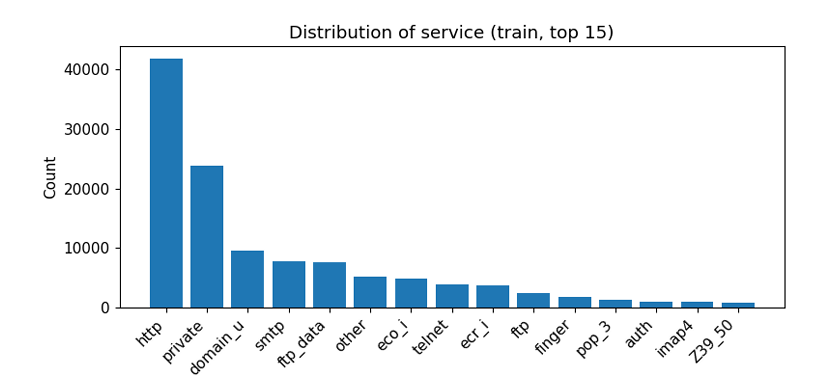
\includegraphics[width=\linewidth]{Figures/methodologyfigures/image5.png}
  \caption{Distribution of the service feature in the training set (top 15 categories). The majority of samples correspond to a small subset of services—most notably HTTP and private—indicating a strong imbalance that affects downstream model learning.}
  \label{fig:image2} 
\end{figure}
 
% image6
% Figure X. Distribution of the flag feature in the training set (top 11 categories). Most connections fall under the SF and S0 flags, while many other flag values occur only sparsely, demonstrating an additional level of categorical imbalance in the NSL-KDD dataset.
\begin{figure}[H]
\centering
  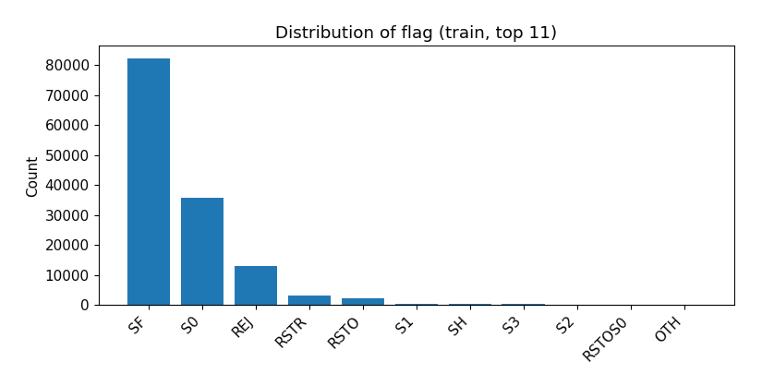
\includegraphics[width=\linewidth]{Figures/methodologyfigures/image6.png}
  \caption{Distribution of the flag feature in the training set (top 11 categories). Most connections fall under the SF and S0 flags, while many other flag values occur only sparsely, demonstrating an additional level of categorical imbalance in the NSL-KDD dataset.}
  \label{fig:image2} 
\end{figure}


\lipsum[1]

% image7
% Figure X. Class distribution in the NSL-KDD training and test sets. The Normal and DoS classes dominate the dataset, while R2L and especially U2R remain severely underrepresented, posing challenges for deep learning–based intrusion detection.

\begin{figure}[H]
\centering
  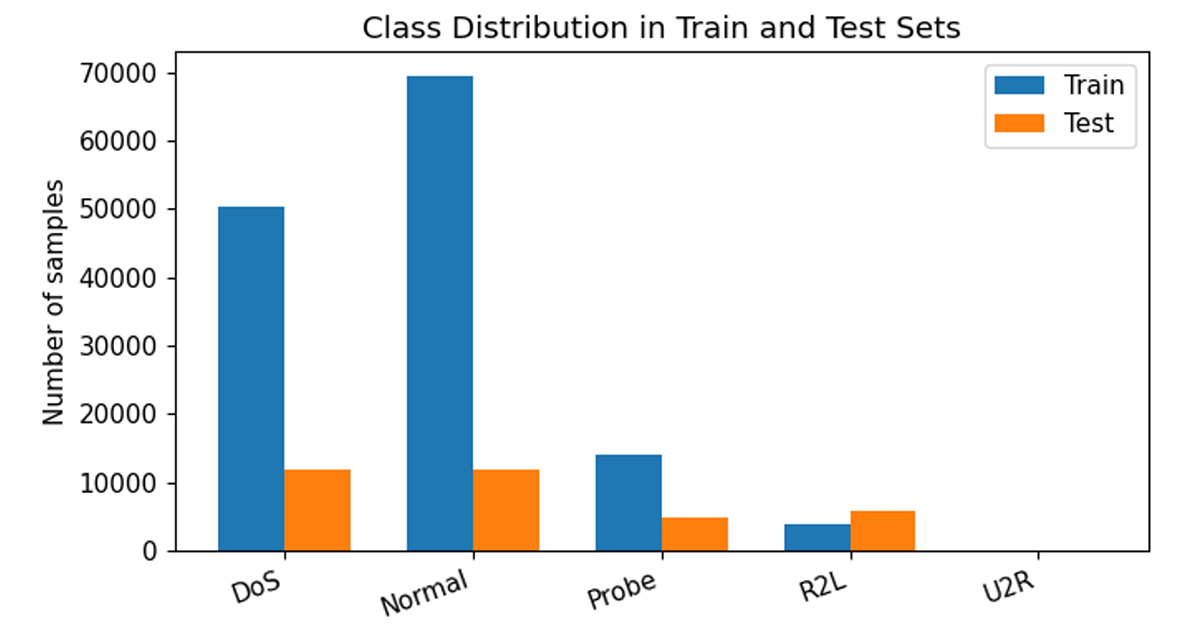
\includegraphics[width=\linewidth]{Figures/methodologyfigures/image7.png}
  \caption{Class distribution in the NSL-KDD training and test sets. The Normal and DoS classes dominate the dataset, while R2L and especially U2R remain severely underrepresented, posing challenges for deep learning–based intrusion detection.}
  \label{fig:image2} 
\end{figure}

\lipsum[1]